\subsection{Age profile of public transfer}
Like other advanced economies, public transfers in Canada are a significant component of inter-generational transfers, complementing transfers between family members.
Through public transfers, individuals transfer wealth from their productive ages to finance consumption during the ages of dependency.
In that sense, the NTA method represents a cross-sectional implementation of the life-cycle hypothesis \citep{andoLifeCycleHypothesis1963,Deaton:2005vr}.
According to that hypothesis, Net Transfer is positive at younger ages when the individual depends significantly on inflows for consumption and outflows are at their lowest levels.
In adulthood, outflows surpass inflows, and Net Transfer becomes negative as the individual engages in income-producing activities.
Finally, in retirement, the individuals return to the government to finance (partially) the remaining years of their lives.
The net transfer becomes positive again and increases to reach its maximum in the final years of life. \autoref{fig:txAge2015}-A shows the age profile of public transfer in Canada for 2015 at the individual level.

\vspace{0.7em}\par
Per-capita inflows are pretty similar for natives and immigrants of almost all ages.
They average \$\numUp{Inflows2015AveYoung019} between birth and age 19, decrease to about \$\numUp{Inflows2015AveAdult2059} between age 20 and 59, and increase by \$\numUp{2015rate60+} for each birthday from age 60 to reach a maximum of \$\numUp{Inflows2015Ave90} just before death.
Despite this similarity, there are slight differences between immigrants and natives, first from age 60 to 70 in favor of immigrants (i.e., they cost less) and then from age 80 to 90 in favor of natives.
While the reasons for the latter are less evident, the former is probably related to later retirement among immigrants as they tend to retire about two years later than natives \citep[p~284]{statCan:006}.

\vspace{0.7em}\par
Like inflows, the age profile of outflows overlaps for immigrants and natives before age 15, as individuals from both groups have almost no income-producing activity during that period.
Beginning at age 15, however, outflows are much lower for immigrants than natives.
From \$\numUp{Outflows2015Immigrants15} for immigrants and \$\numUp{Outflows2015Natives15} for natives at age 15, outflows increase rapidly, and the trends diverge for the two groups.
Between age 35 and 59, contributions stabilized around \$\numUp{Outflows2015AveAdult3554Immigrants} for immigrants and \$\numUp{Outflows2015AveAdult3554Natives} for natives.
However, the gap slightly reduces while outflows decrease steadily between ages 55 and 69.
Thereafter, till the end of life, contributions stabilized around \$\numUp{Outflows2015AveAdult70Immigrants} for immigrants and \$\numUp{Outflows2015AveAdult70Natives} for natives.

\vspace{0.7em}\par
While the per-capita profiles are different but pretty close for immigrants and natives in 2015, the aggregate profile illustrated in \autoref{fig:txAge2015}-B shows different patterns for the two populations, mainly due to the difference in their population size.
For instance, natives are responsible for most public transfers at all ages, especially for the sub-population under ten and between 60 and 70 years old. These are the ages where the size gap between the two populations is the largest.

\begin{figure}[H]%
  \caption{Age profile of public transfer for immigrants and natives, Canada 2015}
  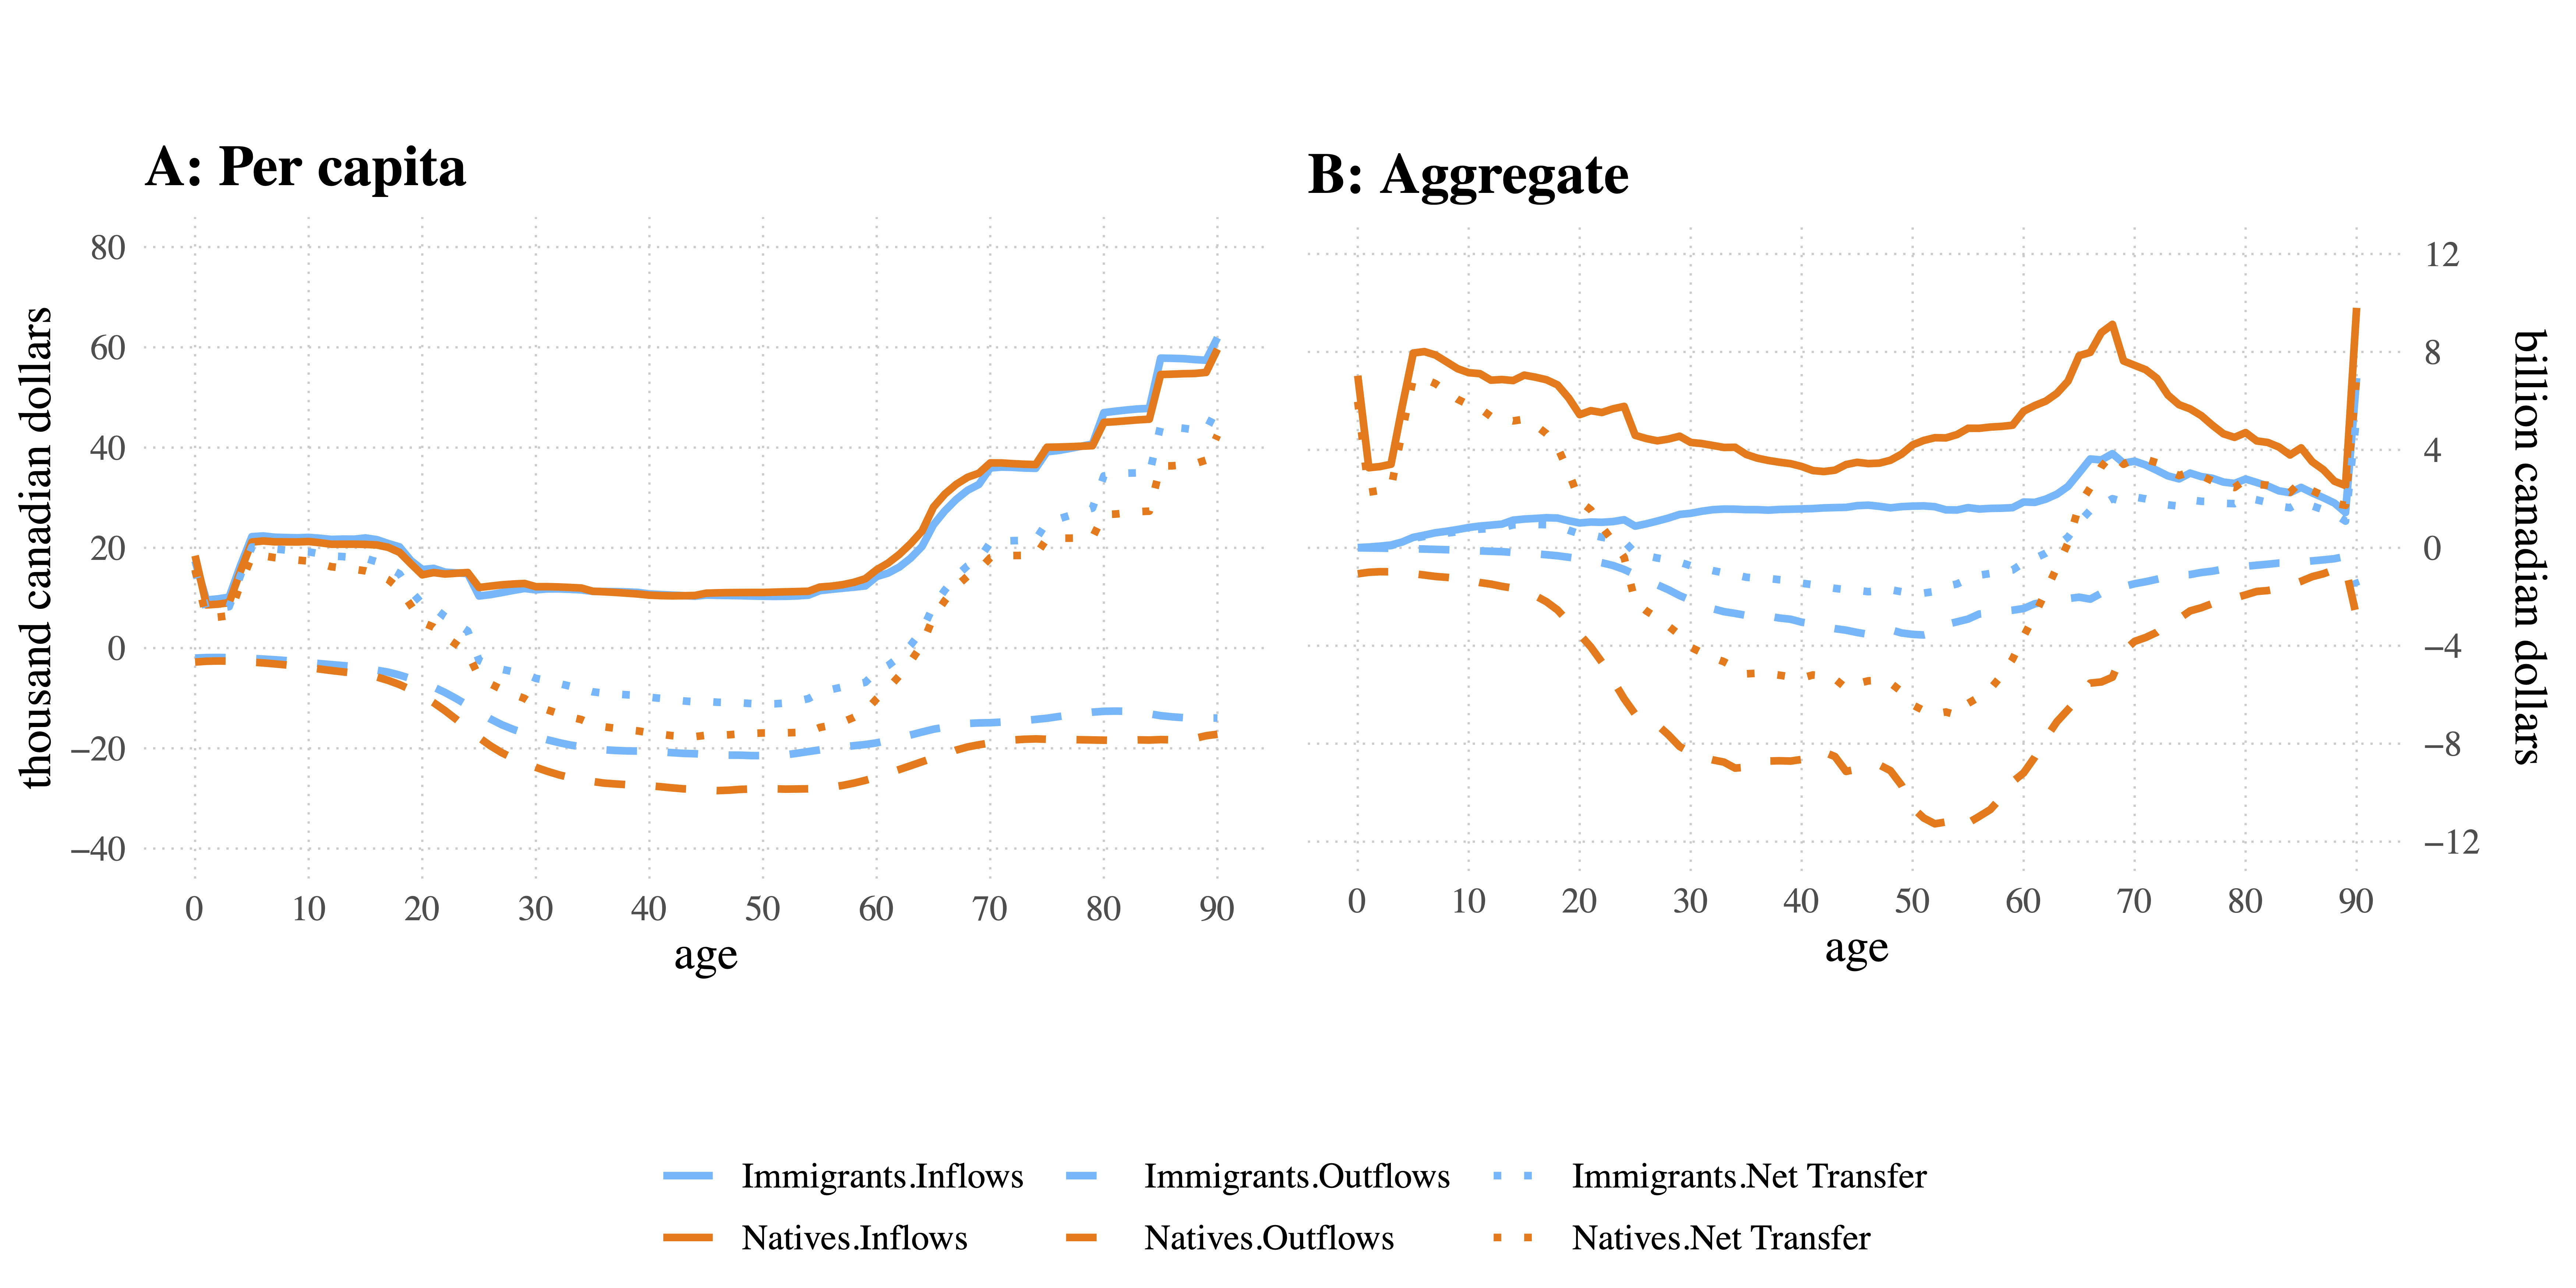
\includegraphics[width=1\textwidth]{../ntaImmig/res/txAge2015.png}%
  \alt{In 2015, per capita inflows were nearly identical for immigrants and natives. However, a noticeable difference in outflow occurs, especially in adult and older age groups, with immigrants contributing less than natives}
  \label{fig:txAge2015}%
\end{figure}%

\subsection{Public transfers in sub-accounts}
Results from \autoref{fig:txAge2015} suggest that immigrants are responsible for a relatively small part of public transfers compared to natives.
However, they account for a disproportionate share of transfer in various sub-accounts compared to their population share.
\autoref{tab:tx2015} splits the Inflow and Outflow transfers for 2015 into their respective sub-accounts along with the population shares for immigrants and natives.
It shows that immigrants represent about 24.2\% of the Canadian population but contribute to 22.7\% of outflows.
Furthermore, while their share in inflow transfers (25.2\%) is much closer to their share in the population, there is a significant gap between inflow sub-accounts.
For instance, immigrants are only responsible for 14.5\% of education costs but account for 29.5\% of health expenses.
For outflow accounts, the share ranges from 21.7\% for sales taxes at one end and 25.4\% for social insurance contributions at the other end.
In dollar values, Net Transfer to public finances in 2015 is positive (\$ \num{19004} million or 0.96\% of GDP) for immigrants but is slightly negative (\$\num{7120} million or 0.36\% of GDP) for natives.
However, as the benefits of immigration become visible only in the medium and long term \citep{Goldin:2011tg}, a more accurate analysis requires a comparison over many years.

  \begin{table}[H]%
    \caption{Population and aggregated public transfers, Canada 2015}
    \alt{Author's calculations}
    \label{tab:tx2015}%
    \begin{center}
      \resizebox{1\textwidth}{!}{%
      \begin{threeparttable}
        %latex.default(tab2015, file = file.path(path, "Docs/ntaImmig/res/tab2015.tex"),     booktabs = TRUE, collabel.just = c("l", "r", "r", "r", "r",         "r"), col.just = c("l", "r", "r", "r", "r", "r"), center = "none",     rowname = NULL, table.env = FALSE, longtable = FALSE, cgroup = c("",         "Absolute numbers", "Percentage"), n.cgroup = c(1, 3,         2), dcolumn = TRUE, )%
\newcolumntype{.}{D{.}{.}{-1}}
\begin{tabular}{lcD{.}{.}{-1}rrcD{.}{.}{-1}D{.}{.}{-1}}
\toprule
\multicolumn{1}{c}{\bfseries }&\multicolumn{1}{c}{\bfseries }&\multicolumn{3}{c}{\bfseries Absolute numbers}&\multicolumn{1}{c}{\bfseries }&\multicolumn{2}{c}{\bfseries Percentage}\tabularnewline
\cline{3-5} \cline{7-8}
\multicolumn{1}{l}{Items}&\multicolumn{1}{c}{}&\multicolumn{1}{r}{Canada}&\multicolumn{1}{r}{Natives}&\multicolumn{1}{r}{Immigrants}&\multicolumn{1}{c}{}&\multicolumn{1}{r}{Natives}&\multicolumn{1}{r}{Immigrants}\tabularnewline
\midrule
\textbf{Population}&&~35065&26575&8490&&~75.8&~24.2\tabularnewline
&&&&&&&\tabularnewline
\textbf{Inflows Transfers}&&638972&478204&160768&&~74.8&~25.2\tabularnewline
\quad Cash transfers (Cash)&&228722&165925&62797&&~72.5&~27.5\tabularnewline
\quad Education Cost (Education)&&~97209&83130&14079&&~85.5&~14.5\tabularnewline
\quad Health Expenses (Health)&&154292&108837&45455&&~70.5&~29.5\tabularnewline
\quad Other Inflows (Others)&&158749&120312&38437&&~75.8&~24.2\tabularnewline
\quad &&&&&&&\tabularnewline
\textbf{Outflows Transfers}&&627472&485325&142147&&~77.3&~22.7\tabularnewline
\quad Contributions to social insurance plans (Insurance)&&~93238&69580&23658&&~74.6&~25.4\tabularnewline
\quad Taxes on Products and Imports (Sales)&&235613&184420&51193&&~78.3&~21.7\tabularnewline
\quad Person Income Taxes (Income)&&238391&186447&51944&&~78.2&~21.8\tabularnewline
\quad Corporate Taxes (Business)&&~68197&51040&17157&&~74.8&~25.2\tabularnewline
\quad Other Outflows (Others)&&~-7968&-6163&-1805&&~77.3&~22.7\tabularnewline
\quad &&&&&&&\tabularnewline
\textbf{Inflows minus Outflows (Net Transfer)}&&~11500&-7120&18620&&-61.9&161.9\tabularnewline
\bottomrule
\end{tabular}
%
        \begin{tablenotes}
          \small
          \item [.] Population are in thousand of persons
          \item [.] Transfer values are in millions of CAD\$
       \end{tablenotes}
     \end{threeparttable}
      }
   \end{center}
\end{table}%
